\section {Ни одного корня внутри промежутка}

Расположение двух корней вне промежутка (Вариант $III$) допускает границы четырёх типов:

\begin {enumerate} [labelindent=\parindent, leftmargin=*]
    \item {$[\alpha, \beta]$}
    \item {$[\alpha, \beta)$}
    \item {$(\alpha, \beta]$}
    \item {$(\alpha, \beta)$}
\end {enumerate}

Для типов границ 2--4 возможны два особых случая:

\begin {itemize}
    \item {существует два корня, при этом один из них попадает в выколотый конец промежутка}
    \item {существует ровно один корень, который попадает либо в выколотый конец промежутка, либо
     за его пределы }
\end {itemize}

\subsection {Границы 2 типа}

Например, особым случаям 2 типа границ будет соответствовать следующая ситуация:

\begin {figure}[h]
    \begin {minipage} [t] {0.5\linewidth}
        \centering
        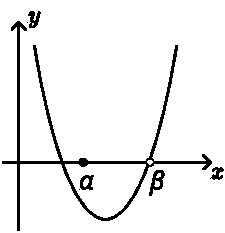
\includegraphics [width=0.6\linewidth] {images/image_06.pdf}
    \end {minipage}
    \begin {minipage} [t] {0.5\linewidth}
        \centering
        \includegraphics [width=0.6\linewidth] {images/image_18.pdf}
    \end {minipage}
\end {figure}

\subsubsection {Первый особый случай}

Чтобы обработать первый особый случай, нужно рассмотреть прохождение параболы $y = f(x)$ через
точку $\beta$. То есть решить уравнение:

\begin {equation*}
    f(\beta) = 0
\end {equation*}


Далее, подставить полученные значения параметра $p$ в трёхчлен $f(x)$ и выбрать параметры, при
которых второй корень существует и лежит за пределами промежутка $[\alpha, \beta)$.  Это можно
сделать с помощью теоремы Виета или проверки соответствующего условия:

       $$ a \cdot f(\alpha) < 0 $$

\subsubsection {Второй особый случай}

Чтобы обработать второй особый случай, нужно рассмотреть равенство дискриминанта нулю, подставить
полученные значения параметра $p$ в трёхчлен $f(x)$ и выбрать параметры, при которых $x_0$ не
попадает внутрь промежутка. Это можно сделать с помощью соответствующего условия:

\begin {equation*}
    \left[
        \begin {aligned}
            x_0 \geqslant \beta
            \\
            x_0 < \alpha
        \end {aligned}
    \right.
\end {equation*}

\subsection {Границы 1 типа. Общий случай}

\begin {figure}[h]
    \begin {minipage} [t] {0.5\linewidth}
        \centering
        \includegraphics [width=0.6\linewidth] {images/image_08.pdf}
    \end {minipage}
    \hfill
    \begin {minipage} [t] {0.5\linewidth}
        \centering
        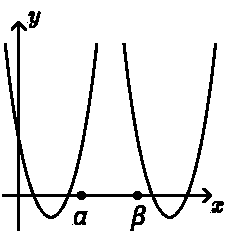
\includegraphics [width=0.6\linewidth] {images/image_09.pdf}
    \end {minipage}
\end {figure}

Чтобы отрезок $[\alpha, \beta]$ лежал внутри параболы, необходимо выполнение следующих условий:

\begin {itemize}
    \item {существует два корня}
    \item {на концах промежутка значения квадратного трёхчлена отрицательны (с точностью до
        умножения на коэффициент $a$)}
\end {itemize}

А чтобы оба корня уравнения находились справа или слева от отрезка, необходимо выполнение следующих
условий:

\begin {itemize}
    \item {существует два корня}
    \item {вершина параболы левее левого конца отрезка или правее правого}
    \item {значения функции в этих концах отрезка положительно (с точностью до умножения на
           коэффициент $a$) }
\end {itemize}

Получаем следующую совокупность трёх систем:

\begin {equation*}
    \left[
        \begin {gathered}
            \begin {cases}
                a \cdot f(\alpha) < 0
                \\
                a \cdot f(\beta) < 0
            \end {cases}
            \\
            \begin {cases}
                D > 0
                \\
                x_0 < \alpha
                \\
                a \cdot f(\alpha) > 0
            \end {cases}
            \\
            \begin {cases}
                D > 0
                \\
                x_0 > \beta
                \\
                a \cdot f(\beta) > 0
            \end {cases}
        \end {gathered}
    \right.
\end {equation*}

Как уже говорилось, чтобы получить полное решение, нужно объединить особые случаи с общим решением
задачи.
